\begin{mainquestion}{parallelrlc}{Parallel RLC Circuit}

\questionpoints
Consider the current-driven parallel RLC circuit shown below.

\begin{center}
\begin{circuitikz}[american voltages]
    \draw (0,0) to[I, l=$I_s$] (0,3) -- (6,3);
    \draw (0,0) -- (6,0);
    \draw (2,3) to[R, l=$R$] (2,0);
    \draw (4,3) to[L, l=$L$] (4,0);
    \draw (6,3) to[C, l=$C$, v={$V_{out}$}] (6,0);
\end{circuitikz}
\end{center}

% =========================================================
\begin{partquestion}{deriveimpedance}
{Derive the impedance $Z$ facing the current source. Express your answer explicitly as the sum of the real and imaginary part.}

\begin{answer}[2.5in]
        The components are in parallel, so we sum their admittances ($Y$):
        \[Y = Y_R + Y_L + Y_C = \frac{1}{R} + \frac{1}{j\omega L} + j\omega C\]
        
        Group the imaginary terms:
        \[Y = \frac{1}{R} + j\left(\omega C - \frac{1}{\omega L}\right)\]
        
        The impedance is $Z = \frac{1}{Y}$. To split into real and imaginary parts, we multiply numerator and denominator by the complex conjugate of $Y$, which is $\frac{1}{R} - j\left(\omega C - \frac{1}{\omega L}\right)$:
        
        \[Z = \frac{1}{\frac{1}{R} + j\left(\omega C - \frac{1}{\omega L}\right)} \cdot \frac{\frac{1}{R} - j\left(\omega C - \frac{1}{\omega L}\right)}{\frac{1}{R} - j\left(\omega C - \frac{1}{\omega L}\right)}\]
        
        \[Z = \frac{\frac{1}{R} - j\left(\omega C - \frac{1}{\omega L}\right)}{\left(\frac{1}{R}\right)^2 + \left(\omega C - \frac{1}{\omega L}\right)^2}\]
        
        Splitting explicitly into Real and Imaginary parts:
        \[Z = \underbrace{\frac{\frac{1}{R}}{\left(\frac{1}{R}\right)^2 + \left(\omega C - \frac{1}{\omega L}\right)^2}}_{\text{Real Part}} - j \underbrace{\frac{\left(\omega C - \frac{1}{\omega L}\right)}{\left(\frac{1}{R}\right)^2 + \left(\omega C - \frac{1}{\omega L}\right)^2}}_{\text{Imaginary Part}}\]
\end{answer}

\end{partquestion}

% =========================================================
\begin{partquestion}{maxmagnitude}
{At what frequency is the magnitude of the impedance $|Z|$ a maximum? What is the phase angle at that frequency?}

\begin{answer}[1.5in]
        The magnitude $|Z|$ is maximized when the denominator of the Real/Imaginary expressions is minimized. The term $\left(\frac{1}{R}\right)^2$ is constant, so we minimize $\left(\omega C - \frac{1}{\omega L}\right)^2$.
        
        This occurs when the imaginary part of the admittance is zero (Resonance):
        \[\omega C - \frac{1}{\omega L} = 0 \implies \omega^2 = \frac{1}{LC} \implies \omega_0 = \frac{1}{\sqrt{LC}}\]
        
        At this frequency $\omega_0$, the impedance is purely real:
        \[Z(\omega_0) = \frac{1/R}{(1/R)^2 + 0} = R\]
        
        Since $Z$ is purely real ($R$), the phase angle is **$0^\circ$**.
\end{answer}

\end{partquestion}

% =========================================================
\begin{partquestion}{extremephase}
{What is the phase angle of the impedance at zero (DC) and at extremely high frequency? Provide an intuitive explanation.}

\begin{answer}[2in]
        \begin{itemize}
            \item \textbf{DC ($\omega \to 0$):} 
            \[Z_L = j\omega L \to 0 \quad (\text{Short Circuit})\]
            The inductor dominates the parallel combination because it has the lowest impedance (0). The current flows entirely through the inductor.
            \[Z_{eq} \approx j\omega L\]
            Since it looks like an inductor, the phase approaches **$+90^\circ$**.

            \item \textbf{High Freq ($\omega \to \infty$):} 
            \[Z_C = \frac{1}{j\omega C} \to 0 \quad (\text{Short Circuit})\]
            The capacitor dominates because it has the lowest impedance (0). The current flows entirely through the capacitor.
            \[Z_{eq} \approx \frac{1}{j\omega C} = -j\frac{1}{\omega C}\]
            Since it looks like a capacitor, the phase approaches **$-90^\circ$**.
        \end{itemize}
\end{answer}

\end{partquestion}

% =========================================================
\begin{partquestion}{bodeplots}
{Let $L=1~mH$, $R=7~k\Omega$, and $C=1~nF$. Create Bode plots for both the magnitude and phase of the transfer function $Z(s)$. \\
    \textbf{Note:} You are encouraged to use MATLAB or other plotting tools to generate these plots if calculating by hand is difficult.}

\begin{answer}[4.5in]
        The resonant frequency is $\omega_0 = \frac{1}{\sqrt{LC}} = \frac{1}{\sqrt{10^{-3} \cdot 10^{-9}}} = \frac{1}{\sqrt{10^{-12}}} = 10^6$ rad/s.
        
        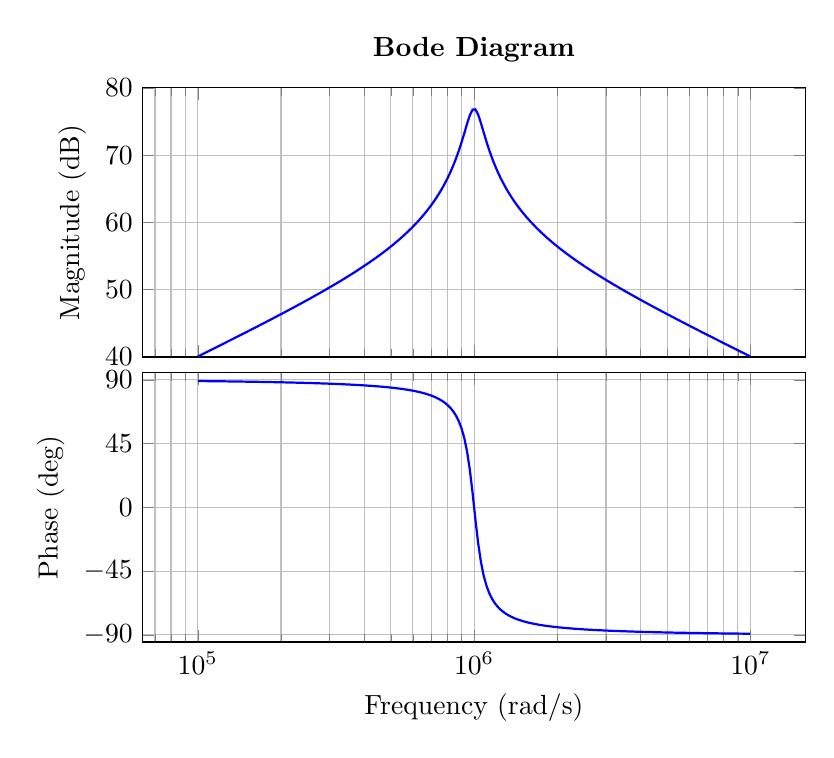
\begin{tikzpicture}
            % Magnitude Plot
            \begin{axis}[
                name=magplot,
                width=10cm, height=5cm,
                xmode=log,
                title=\textbf{Bode Diagram},
                ylabel={Magnitude (dB)},
                ymin=40, ymax=80,
                grid=both,
                xticklabels=\empty
            ]
            % Function: 20*log10( 1 / sqrt( (1/7000)^2 + (x*1e-9 - 1/(x*1e-3))^2 ) )
            % We plot from 10^5 to 10^7 rad/s centered on resonance 10^6
            \addplot[blue, thick, domain=1e5:1e7, samples=200] {20*log10( 1 / sqrt( (1/7000)^2 + (x*1e-9 - 1/(x*1e-3))^2 ) )};
            \end{axis}
            
            % Phase Plot - Stacked below
            \begin{axis}[
                name=phaseplot,
                at={(magplot.south west)}, anchor=north west, yshift=-0.2cm,
                width=10cm, height=5cm,
                xmode=log,
                ylabel={Phase (deg)},
                xlabel={Frequency (rad/s)},
                ymin=-95, ymax=95,
                ytick={-90, -45, 0, 45, 90},
                grid=both
            ]
            % Phase = - degrees( atan( (wC - 1/wL) / (1/R) ) ) = - atan( (wC - 1/wL) * R )
            \addplot[blue, thick, domain=1e5:1e7, samples=200] {-atan( (x*1e-9 - 1/(x*1e-3)) * 7000 )};
            \end{axis}
        \end{tikzpicture}
        
        \vspace{0.5em}
        MATLAB Code used to verify:\\
        \texttt{L = 1e-3; R = 7e3; C = 1e-9;}\\
        \texttt{num = [L 0];}\\
        \texttt{den = [L*C L/R 1];}\\
        \texttt{bode(num, den);}
\end{answer}

\end{partquestion}

\end{mainquestion}
